\begin{figure}
	\begin{center}
		\begin{tikzpicture}[sibling distance=8pt]
		\Tree[
		.B A [ .C \edge[blank]; \node[blank]{}; D ]
		]
		\node at (0,1) {Version 1};
		\end{tikzpicture}
		\qquad\hspace{40mm}
		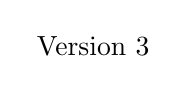
\begin{tikzpicture}[sibling distance=8pt]
		\Tree[
		.B A [ .D C E ]
		]
		\node at (0,1) {Version 3};
		\end{tikzpicture}
	\end{center}
\raggedcolumns
\begin{multicols}{2}
\centering
\footnotesize
\begin{vdTable}{Vertex}
	Version & Left & Right   & Key & Value
\end{vdTable}
\begin{vdTable}{A}
	1 & $\Lambda$ & $\Lambda$ & 10 & 5 \\
	2 & $\Lambda$ & $\Lambda$ & 10 & 6
\end{vdTable}
\begin{vdTable}{B}
	1 & A & C & 20 & 15 \\
	3 & A & D & 20 & 15
\end{vdTable}
\begin{vdTable}{C}
	1 & $\Lambda$ & D & 30 & 27 \\
	3 & $\Lambda$ & $\Lambda$ & 30 & 27
\end{vdTable}
\begin{vdTable}{D}
	1 & $\Lambda$ & $\Lambda$ & 40 & 39 \\
	3 & C & E & 40 & 39
\end{vdTable}
\begin{vdTable}{E}
	3 & $\Lambda$ & $\Lambda$ & 50 & 99
\end{vdTable}\\
\end{multicols}

Tree is shown for version 1 (left) and 3 (right). Internal collections for each vertex are displayed. Operation that created version 2 changed value of key 10. Operation that created version 3 inserted vertex E and triggered a rotation. Faithful to The Art of Computer Programming, $\Lambda$ represents a null pointer.
\caption{A tree with dictionaries in vertices} 

\end{figure}